\documentclass[aspectratio=1610]{beamer}
\usepackage[utf8]{inputenc}
\usepackage[T1]{fontenc}
\usepackage[german]{babel}
\usepackage[useregional]{datetime2}
\usepackage[nameinlink]{cleveref}
\usepackage[section]{placeins}
\usepackage{xcolor}
\usepackage{graphicx}
\usepackage{csquotes}
\usepackage{amsmath} % for $\text{}$
\usepackage{pflichtenheft}
\usepackage{enumitem}
\setlist{nosep}

\newcommand\urlpart[2]{$\underbrace{\text{\texttt{#1}}}{\text{#2}}$}
\raggedbottom
\crefname{figure}{Abb}{Abb}

\newcommand\producttitle{treff.}
\hypersetup{
	pdftitle={Pflichtenheft: \producttitle},
	bookmarks=true,
}


% header & footer
\usepackage{scrlayer-scrpage}
%\lofoot{\today}
%\refoot{\today}
\pagestyle{scrheadings}

\title{
\includegraphics[width = 50mm]{images/logo_crop.png}}
\subtitle{\huge Pflichtenheft}
\author{Lukas Dippon
	\and Jens Kienle
	\and Matthias Noll
	\and Fabian Röpke
	\and Tim Schmidt
	\and Simon Vögele}

\begin{document}
	
	\begin{frame}[plain]
	\maketitle
	\end{frame}

	\begin{frame}[plain]
		\begin{minipage}{0.5\textwidth}
			\setlength{\fboxsep}{0pt}% space between border and image
			\setlength{\fboxrule}{1pt}% width of border
			\fbox{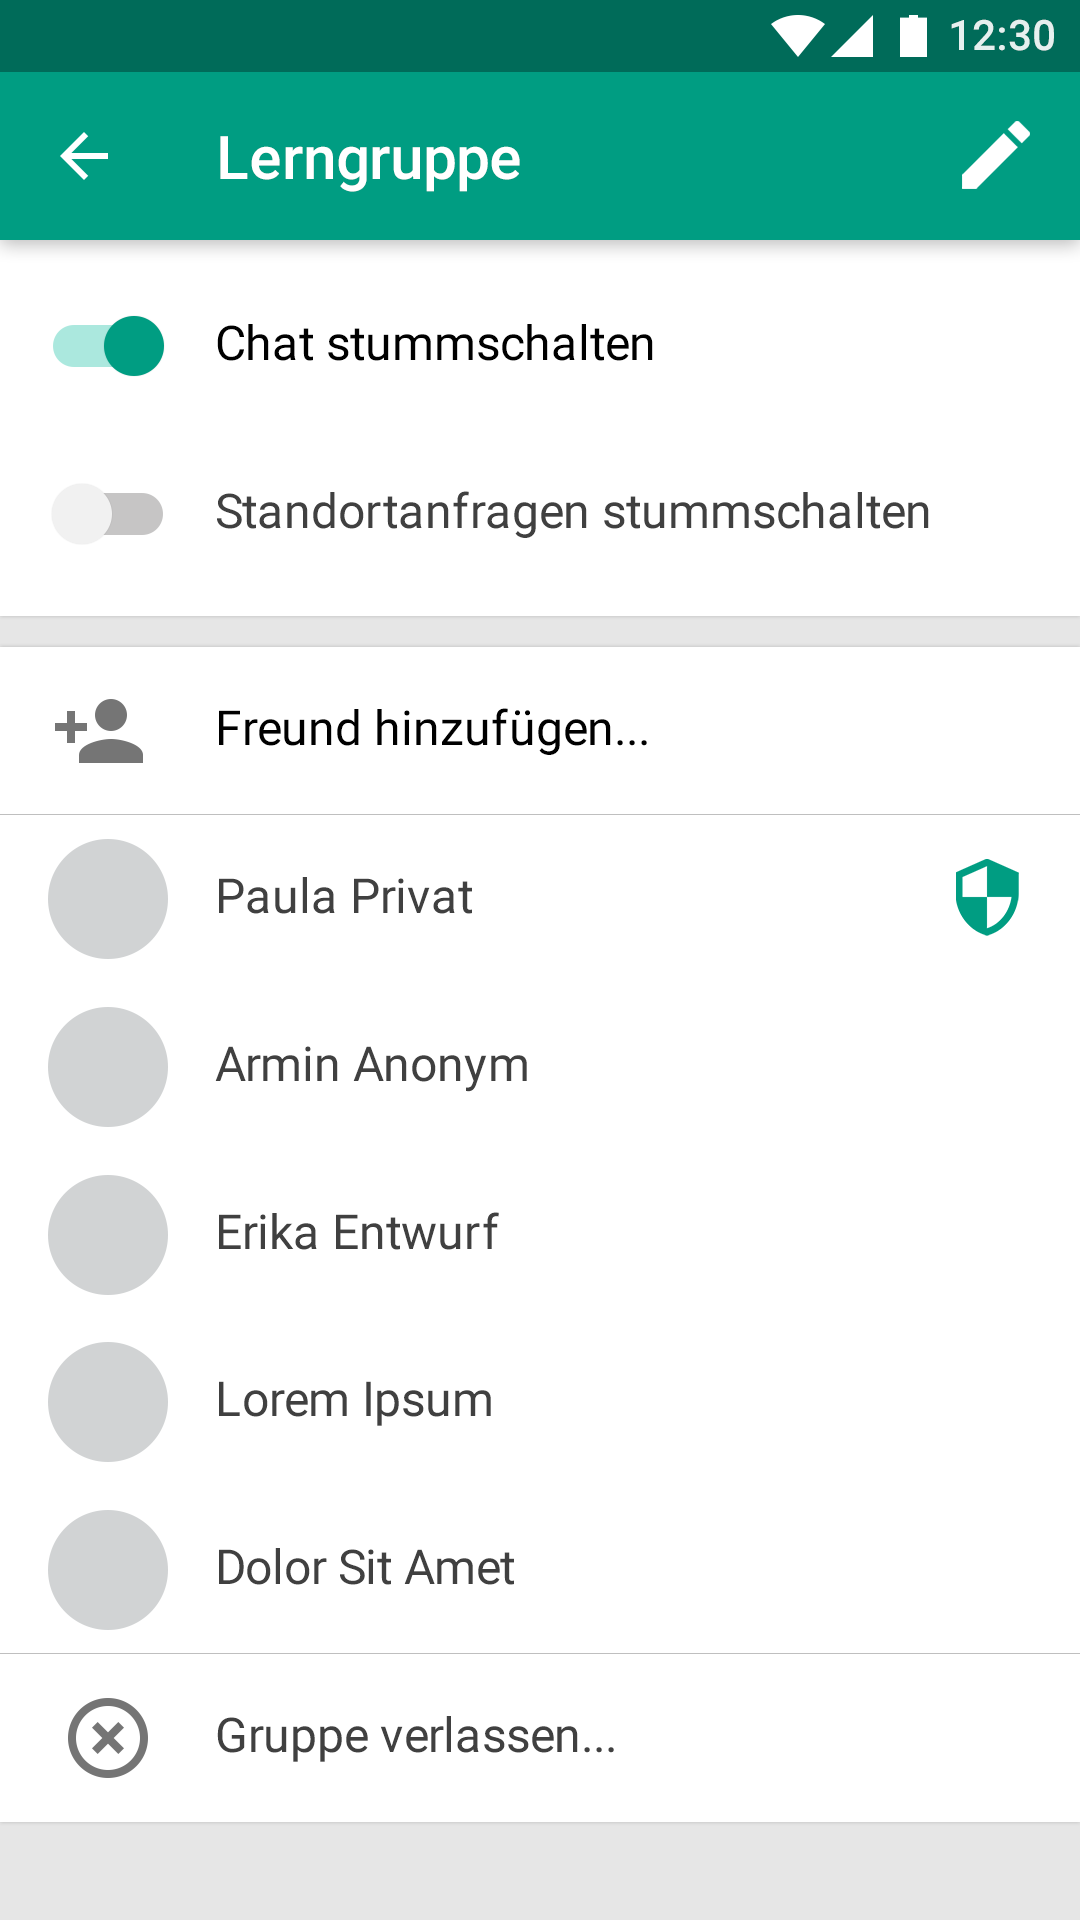
\includegraphics[width = 45mm]{images/gui-mockups/group_members.png}}
			\captionsetup{labelformat=empty}
			\centering
			\captionof{figure}{\textbf{Test}}
		\end{minipage}%
		\begin{minipage}{0.5\textwidth}
			\begin{itemize}
				\item Eine Liste aller Gruppenmitglieder und bla und blkasajsdhkajsdh
				\item test
				\item test
			\end{itemize}
		\end{minipage}
	
	\end{frame}


\end{document}